\subsection{1D Heat Rod}\label{ex:heat-set-sample}

We demonstrate that the same principles at play in Example\ref{ex:decay-set-sample} apply to another nonlinear problem.
Here, the quantification of uncertainty is for the thermal conductivity properties of a material based on temperature data collected after heating it in an experiment.


Consider the one-dimensional heat equation with homogeneous Neumann boundary conditions on the unit interval:

\begin{equation}
\begin{split}
\rho c \frac{\partial T}{\partial t} = \nabla \cdot ( \kappa \nabla T) + f(x), \quad & x\in (0,1), t\in (0,1) \\
f(x) = A e^\frac{- (x-0.5)^2}{w} \Chi_{[0,0.5]}(t)
\end{split}
\end{equation}
\emph{Alternative setup: }

\begin{equation}
\begin{cases}
\rho c \frac{\partial T}{\partial t} = \nabla \cdot ( \kappa \nabla T) + f(x,t), & \text{if } x\in \Omega \\
\frac{\partial T}{\partial \vec{n}} = 0 & \text{if } x\in \partial \Omega
\end{cases}
\end{equation}
where $\Omega = (0,1)\times (0,1)$ is the space-time interior and $f(x,t) = A e^\frac{- (x-0.5)^2}{w} \Chi_{[0,0.5]}(t)$.

Here, we interpret the following problem as heating the middle of an infinitesimally thin unit-length rod for half a second with a heat-source modeled by a Gaussian curve with amplitude $A=50$ and variance of $w=0.05$.
This heat source is turned on at the beginning of the experiment and turned off halfway through the 1-second duration.

The rod is subdivided in two, and each half has an uncertain thermal diffusivity $\kappa \in [0.01, 0.2]$.
This yields a two-dimensional parameter space $\param = (\param_1, \param_2) \in [0.01, 0.2]\times [0.01, 0.2]$, where $\param_1$ represents the thermal diffusion on the left-half and $\param_2$ is the $\kappa$ for the right half.

\begin{figure}[h]
\begin{minipage}{.475\textwidth}
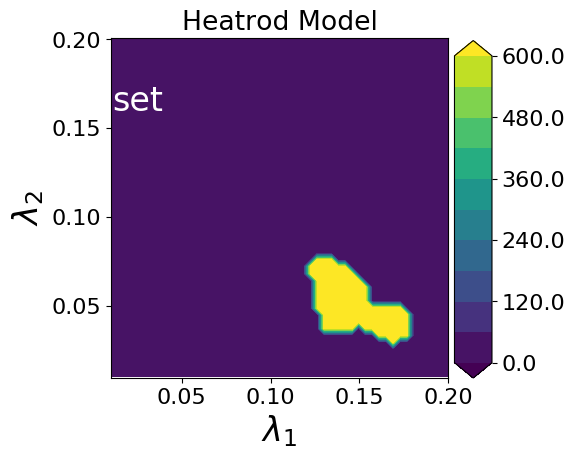
\includegraphics[width=\linewidth]{examples/fig_heatrod_q1/HeatrodModel--set_N50_em.png}
\end{minipage}
\begin{minipage}{.475\textwidth}
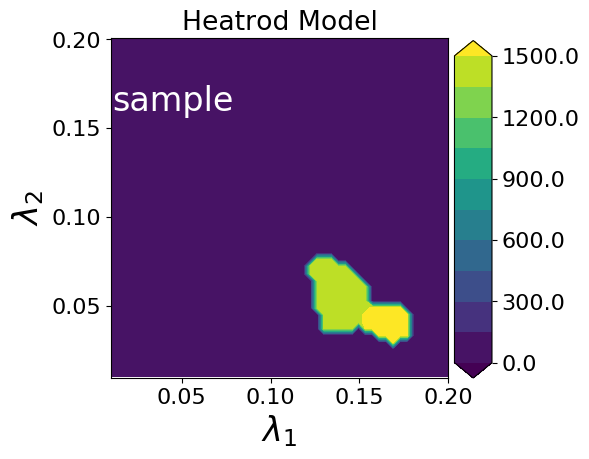
\includegraphics[width=\linewidth]{examples/fig_heatrod_q1/HeatrodModel--sample_N50_mc.png}
\end{minipage}
\caption{The inverse image of the reference measure for set-based (left) and sample-based (right) solutions for $N=50$ parameter samples.}
\label{fig:heatrod-sol-ex}
\end{figure}
